\documentclass{dhbenelux}

% this makes citations #'s but using parentheses. having
% trouble making it use square brackets
%\usepackage{natbib}
%\setcitestyle{numbers}
\usepackage{hyperref}
\usepackage{booktabs} % for toprule, midrule, bottomrule in tables
\usepackage{authblk} % for multiple authors and affiliations
\usepackage{graphicx} % to inlcude graphics with \includegraphics
\usepackage{rotating}
\usepackage{tikz}
%\usepackage{colorlinks=true,linkcolor=blue}{hyperref}%

\setlength{\parindent}{0em}
\setlength{\parskip}{1em}

\author{Shashank Gupta}
\author{Jordan Hamel}
\author{Alex Pirola}
\author{Arjun Prihar}
\author{Agnes Robang}
\author{Anita Zhang}

\affil{APC 524}
\affil{December 20th, 2021}

\title{Tool Suite for Crystal and Bond Properties Analysis }

\begin{document}

\maketitle
% include copright statement on first page:
\thispagestyle{papertitlepage} 

\section{Introduction}

\subsection{Motivation}

Fourier-transform infrared spectroscopy (FTIR) and X-ray diffraction (XRD) are two experimental techniques that are used extensively in the field of materials science to analyze the properties of a given sample. One common application for FTIR and XRD is to confirm the formation of hydration products, such as calcium silicate hydrate (CSH) in Portland Cement (~\cite{shi2019ftir}). Both of these procedures generate graphs with peaks whose position, height, and width help determine the existence and microstructure of phases present in the material. Once the data has been collected, it can be cross-referenced with an existing database that contains the “peak characteristics” and unique label corresponding to each material. However, this matching process is often done manually, which is labor-intensive and less precise than measuring attributes computationally. As such, the ultimate goal of our project was to build a modular tool suite that automates this traditionally laborious process. Though the motivation for this tool comes from the authors' research in cement labs, as the database grows, the software will save a significant amount of time for any researchers who analyze materials.  


\subsection{Scientific Background:}

\subsubsection{X-Ray Diffraction}
\label{X-Ray Diffraction}

X-Ray Diffraction (XRD) is a nondestructive characterization technique for crystalline materials. The test provides information on crystalline structure, crystal orientations, phases, and additional parameters like crystallinity, mean grain size, and crystal defects. The underlying principle is that X-ray wavelengths is of the order of inter-plane spacing in a crystal, hence crystalline structure act as diffraction grating for X-rays (\cite{XRD1}).

Constructive interference between monochromatic X-rays and a crystalline sample is the basis of X-ray diffraction. A cathode ray tube produces the X-rays, which are then filtered to produce monochromatic radiation, collimated to focus the beam, and aimed onto the sample. The constructive interference of the incident rays happens when Bragg's Law is satisfied. Bragg's law relate the lattice spacing (d) and diffraction angle ($\theta$) to the wavelength of X-ray ($\lambda$) (\cite{XRD_Ref2}).

\[ n\lambda = 2dsin(\theta) \]
By scanning the sample through a range of $2\theta$ angles, all possible diffraction directions of the lattice should be attained due to the random orientation of the powdered material. Conversion of the diffraction peaks to d-spacings allows identification of the mineral because each mineral has a set of unique d-spacings. Typically, this is achieved by comparison of d-spacings with standard reference patterns. An illustration of a typical XRD setup is shown in Figure \ref{fig:XRD2}.

\begin{figure}[!h]
    \centering
    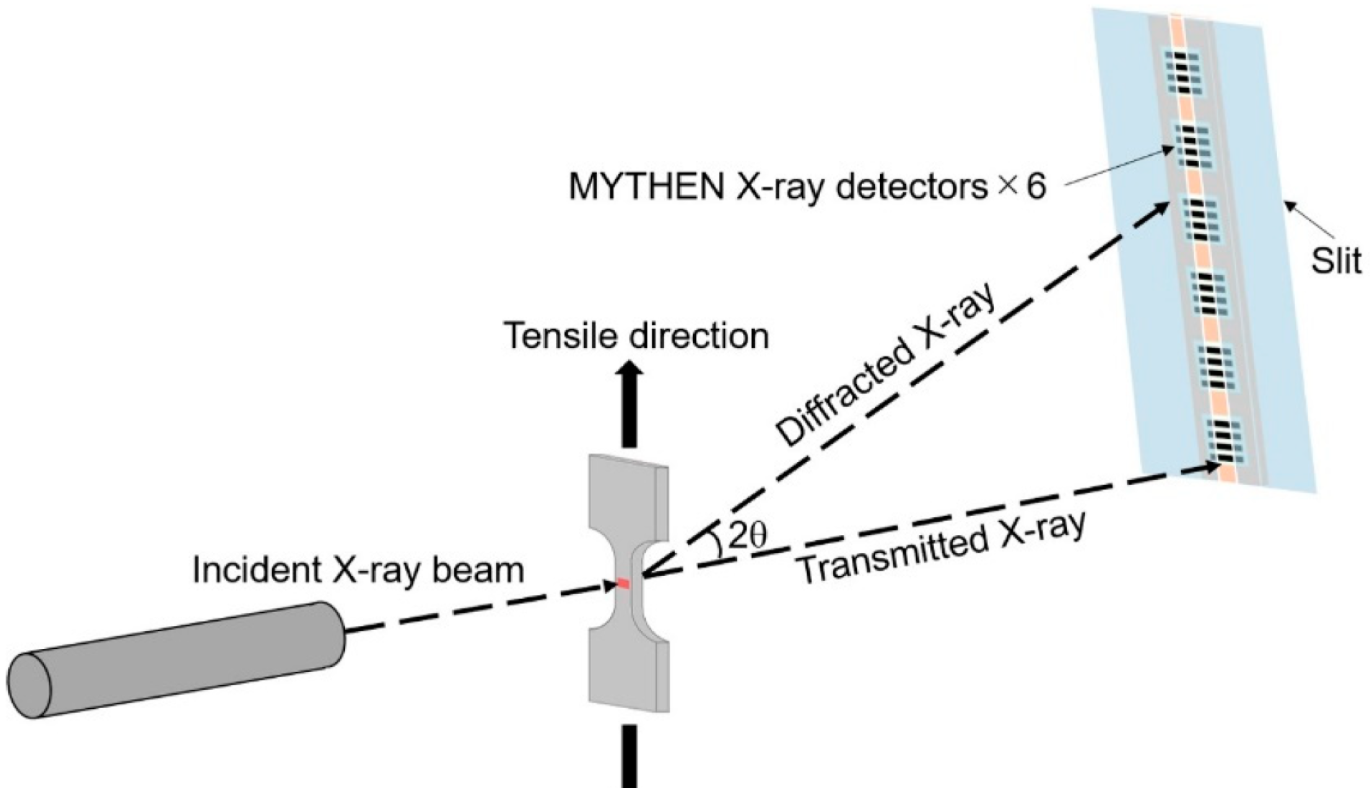
\includegraphics[scale=0.4]{XRD2.PNG}
    \caption{Schematic illustration of the X-ray diffraction (XRD) measurement system (\cite{cryst})}
    \label{fig:XRD2}
    
\end{figure}

 The intensity of diffracted X-rays is continuously recorded as the sample and detector rotate through their respective angles. A peak in intensity occurs when the mineral contains lattice planes with d-spacings appropriate to diffract X-rays at that value of $\theta$. Although each peak consists of two separate reflections ($K_{\alpha1}$ and $K_{\alpha2}$), at small values of 2$\theta$ the peak locations overlap with $K_{\alpha2}$ appearing as a hump on the side of $K_{\alpha1}$. Greater separation occurs at higher values of θ. Typically these combined peaks are treated as one. 

\begin{figure}[!h]
    \centering
    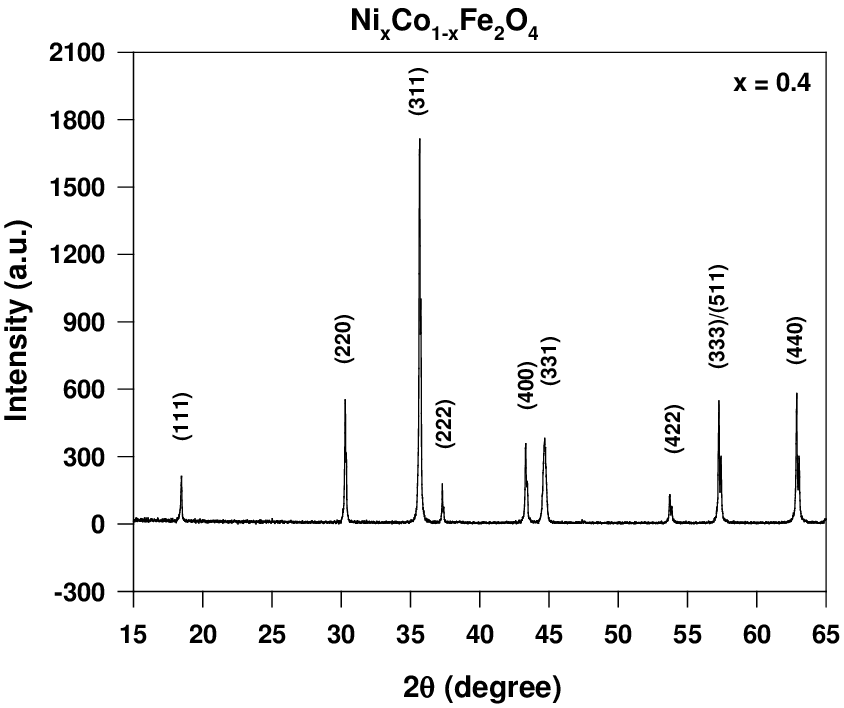
\includegraphics[scale=0.4]{XRD1.PNG}
    \caption{Reference XRD Pattern (\cite{XRD1})}
    \label{fig:XRD1}
    
\end{figure}

Results are commonly presented as peak positions at 2$\theta$ and X-ray counts (intensity) in the form of a table or an x-y plot, as seen in Figure \ref{fig:XRD1}. Intensity (I) is either reported as peak height intensity, that intensity above background, or as integrated intensity, the area under the peak. The relative intensity is recorded as the ratio of the peak intensity to that of the most intense peak.

The d-spacing of each peak is then obtained by solution of the Bragg equation for the appropriate value of $\lambda$. Once all d-spacings have been determined, automated search/match routines (also the segment of our code) compare the d-values of the unknown to those of known materials. Because each mineral has a unique set of d-spacings, matching these d-spacings provides an identification of the unknown sample. A systematic procedure is used by ordering the d-spacings in terms of their intensity beginning with the most intense peak. In our work, we are automating the pattern reading and mineral recognition from the 2$\theta$ vs Intensity values, which will be discussed in greater detail in Section \ref{design} 

\subsubsection{Fourier-Transform Infrared Spectroscopy}

FTIR spectroscopy is a popular technique in the field of materials science for deducing the chemical composition of a sample. FTIR analysis entails shining a polychromatic beam of light (a beam consisting of several frequencies) at a sample and subsequently measuring how much of the beam is absorbed. This process is repeated with different combinations of frequencies and then mapped to spectral information via a transformation that inverts the domain of the raw detector output ("Introduction to fourier", 2001). Mathematically, this transformation is exactly the Fourier transform, which, in this case, converts the domain from mirror displacement to wavelength. See Figure \ref{fig:FTIR_setup} for a typical setup of FTIR analysis. 

\begin{figure}[!h]
    \centering
    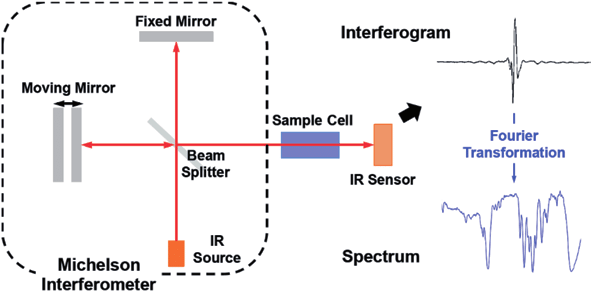
\includegraphics[scale=0.5]{FTIR.png}
    \caption{Schematic of FTIR analysis and data processing. Note that other interferometer configurations exist but Michelson is the most common commercially \cite{FTIR_setup}.}
    \label{fig:FTIR_setup}
    
\end{figure}

Ultimately, the resulting graph displays the sample’s absorbance of the infrared light at various wavelengths which can then be cross-referenced against a database of known materials to gain structural insight about the sample. The procedure for data collection and analysis is quite analogous to that of XRD, described in Section \ref{X-Ray Diffraction}. The underlying principle behind spectroscopy is that the absorbance of a material is uniquely determined by its chemical structure; namely, the shape of molecular bonds, the mass of the atoms, and their associated vibronic coupling will all impact how much light of a certain frequency passes through the material ("FTIR Analysis", 2021). Thus, the resulting peaks in spectra can be leveraged to identify the sample. An example of an FTIR pattern for propylamine is shown below in Figure \ref{fig:FTIR_ex}.

\begin{figure}[!h]
    \centering
    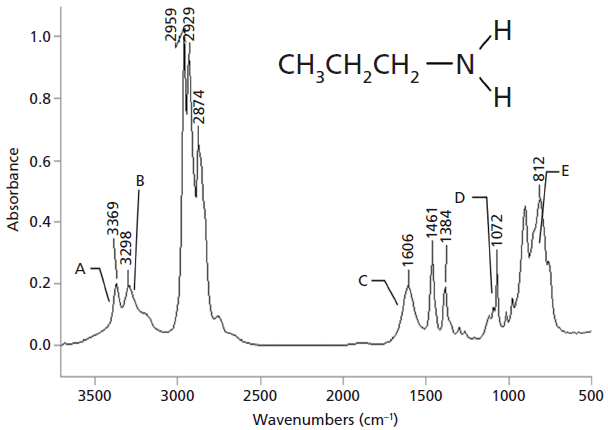
\includegraphics[scale=0.5]{spectroscopy_ex.png}
    \caption{Example of an FTIR pattern for propylamine. \cite{spectroscopy_ex}}
    \label{fig:FTIR_ex}
\end{figure}

\subsubsection{Baseline Removal}

The baseline removal process for the FTIR data relies on an iterative, linear regression of a polynomial curve-fitting function. This method is based on a modified polynomial fit used for Raman Spectra of biological fluorescence (\cite{baseline_removal}). First, a modified Vandermonde matrix is generated with the same number of rows as the input array and columns as the degree of the final fitting polynomial. This matrix is then decomposed using QR factorization, and the resulting Q matrix is used as a target for the linear regression to identify the baseline. The linear regression takes the polynomial coefficients of the Q matrix as training data and the input array as target data, and makes a prediction of the subsequent data point using the training data. For any instance in which the input array has a higher numerical value than the predicted data, the predicted data is saved and the saved data is used to update the input array for each iteration. The program currently defaults the number of iterations to 100. A final baseline is computed and subtracted from the original input data, returning a baseline-removed FTIR spectrum. An example of the procedure and effect of baseline removal is shown below in Figure \ref{fig:baseline}

\begin{figure}[!h]
    \centering
    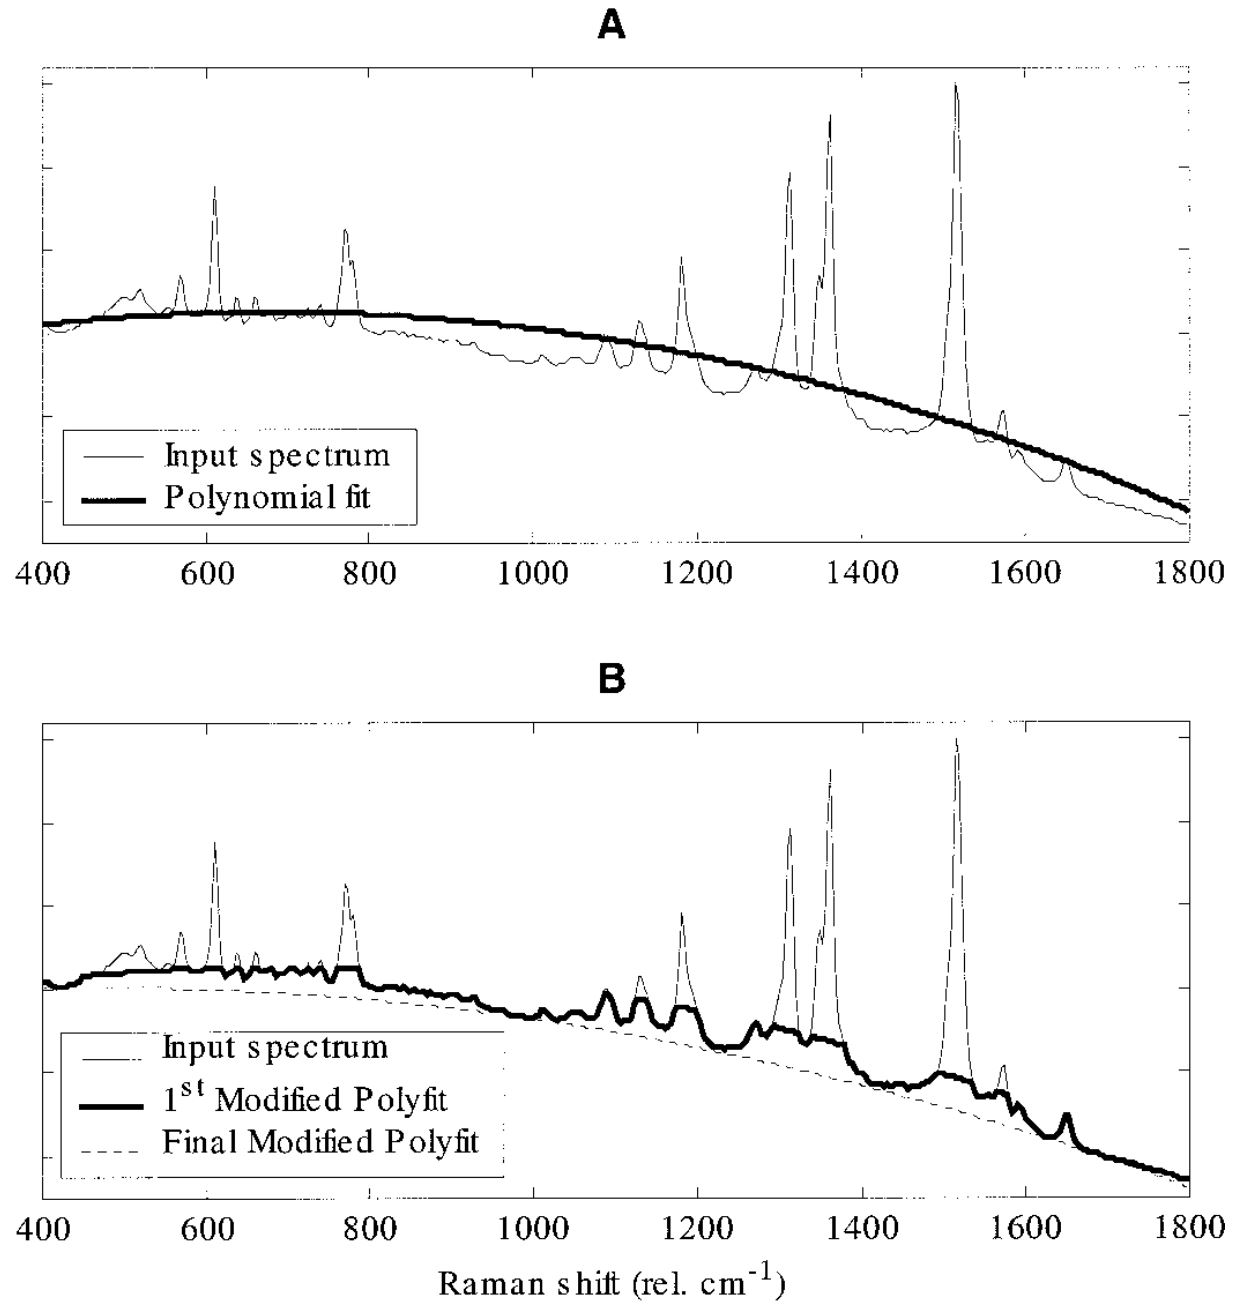
\includegraphics[scale=0.75]{BASELINE FITTING.JPG}
    \caption{Baseline removal method  (\cite{baseline_removal})}
    \label{fig:baseline}
    
\end{figure}

\section{Architectural Design} \label{design}

The project was divided into three main components: analysis methods, database methods, and a driver code. Separate analysis and database methods were required for each technique, XRD and FTIR. So far, we have implemented two methods of XRD analysis: one which relies on standard polynomial fitting via a spline and one which leverages Rietveld analysis to more accurately capture the information contained in overlapping peaks. The FTIR analysis also relies on peak fitting, but has an additional first step of removing the baseline from the data. A baseline removal method has been developed for this analysis suite. 

Ultimately, given some raw XRD or FTIR data, our program performs peak finding/fitting to extract the characteristic peak parameters. Then, we compare this peak information to our database and finally, we return the closest matching material classification. We leverage abstract base classes (ABCs) for both the experimental technique and peak fitting method used. As a result, the driver code is completely agnostic of whether it's processing XRD or FTIR data and whether it's using Rietveld, Pawley, Le-Bail, or standard polynomial fitting to find the peaks. The principal benefit of this is that our pipeline is highly modular and conducive to future modifications that expand the "menu" of options in either of these categories. 

To start, our program accepts seven command-line arguments specifying: the data to be analyzed (as a .csv file), the corresponding experimental technique (FTIR vs XRD), and the peak profile fitting method to be used, along with some keywords. If Rietveld, Pawley, or Le-Bail is the desired method, then two additional arguments are necessary: strategy and peak height threshold, both of which will be discussed in Section \ref{profiling}. Note that the .csv file is expected to have a two-column format; the first column should be 2$\theta$ (degrees) or wavenumber (1/cm) and the second one should be intensity (counts per second) or transmittance (\%), for XRD and FTIR data respectively. The README.txt file in our repository specifies exactly how the input data and command-line arguments should be formatted. Then, the selected peak profile fitting method returns a list of "peak" objects containing the estimated peaks and their corresponding parameters. This list is then used in the CompareToDatabase module which determines the closest matching material. The XRD database was scraped from \href{http://webmineral.com/}{webmineral.com} while the FTIR database was manually transferred from Open Specy (\cite{cowger_gray_hapich_rochman_lynch_primpke_munno_frond_herodotou_2020}). The complete UML diagram can be found in Figure \ref{fig:UML} on the following page. An example command-line input and corresponding output are shown in Figures \ref{fig:input} and \ref{fig:output} below.

\begin{figure}[!h]
    \centering
    \begin{minipage}{0.45\textwidth}
        \centering
        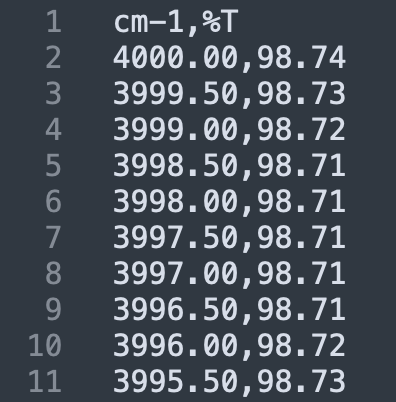
\includegraphics[width=0.9\textwidth]{APC524_input.png} % first figure itself
        \caption{Sample input}
        \label{fig:input}
    \end{minipage}\hfill
    \begin{minipage}{0.45\textwidth}
        \centering
        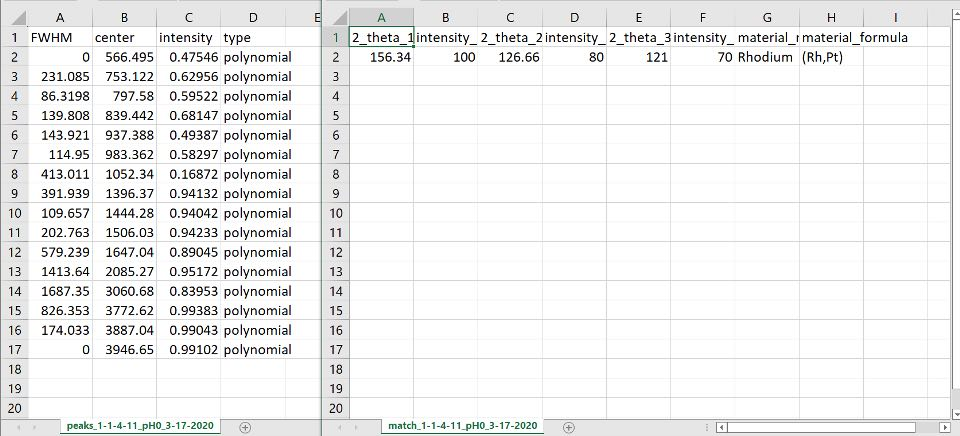
\includegraphics[width=0.9\textwidth]{APC_output.jpg} % second figure itself
        \caption{Corresponding output. Two .csv files, one with peak information and the other with material matches}
        \label{fig:output}
    \end{minipage}
\end{figure}


\begin{sidewaysfigure}[]
    \centering
    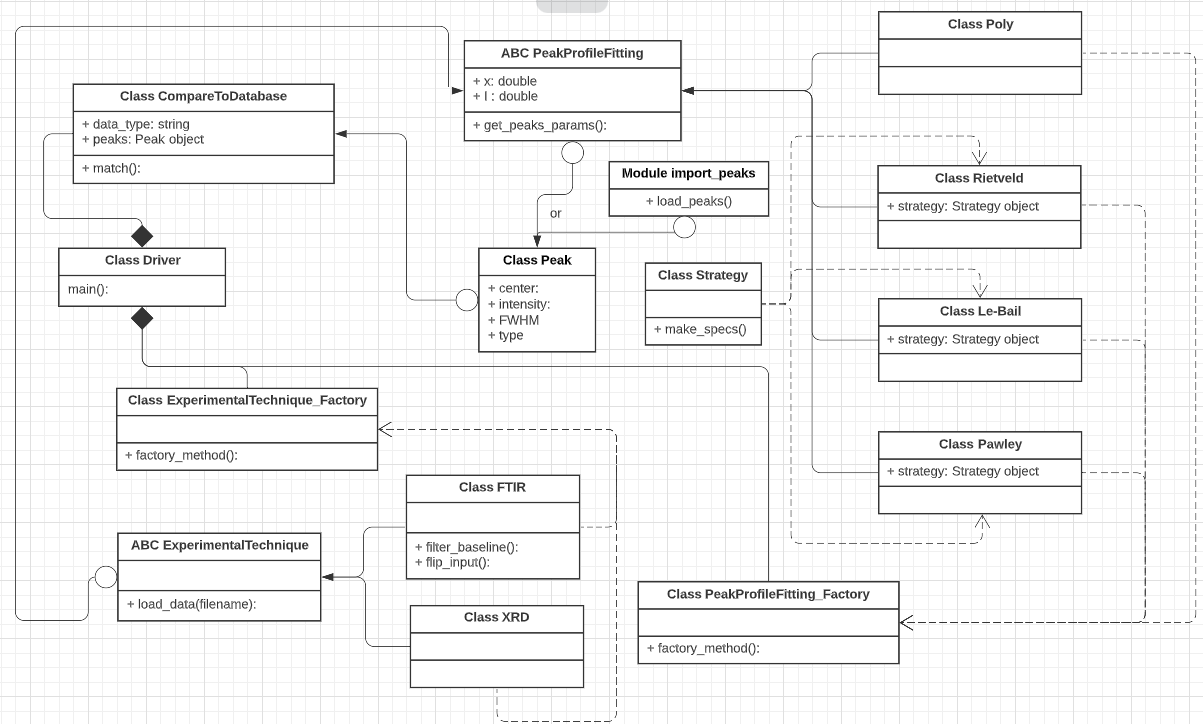
\includegraphics[scale=0.8]{APC_UML.png}
    \caption[UML Diagram]{UML Diagram}
    \label{fig:UML}
\end{sidewaysfigure}

Note that the current program only performs the Rietveld and Polynomial fitting methods, with implementation of Le-Bail and Pawley scheduled as future work. Figure \ref{fig:rietveld_ex} shows the peaks found by the Rietveld method overlaid on top of the original XRD data. The polynomial method is a "quick and dirty" module that fits the raw data using a univariate spline (i.e. combination of polynomials). It's extremely efficient but fails to capture the same detail as a method like Rietveld. 

It's also important to note that although our program was intended to be used as a complete end-to-end pipeline, it is also highly modular and capable of functioning as a library if the user would like to execute any of the above steps independently. This would be done by simply importing the relevant class to ensure datatype compatibility (e.g. to convert the user's pre-existing 2-D array of peak parameters to a list of peak objects).

\begin{figure}[!h]
    \centering
    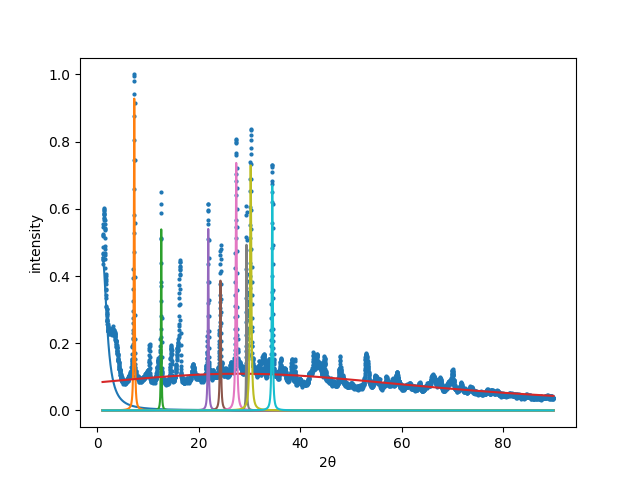
\includegraphics[scale=0.7]{figure1 for presentation.png}
    \caption{Results of Rietveld Analysis of XRD data}
    \label{fig:rietveld_ex}
\end{figure}


\section{Development Process} \label{dev_process}

\subsection{Logistics}
After submitting our preliminary design document, our group had an initial in-person meeting to finalize the vision for our program and have an open conversation about how we all wanted to work together. For example, we all agreed to use GroupMe to coordinate our development efforts and that overcommunication would be a better problem to have than the opposite. All subsequent meetings were virtual and took place over Zoom. 

Our current pipeline can be divided into five main pieces of code: two peak fitting methods, two databases, and the driver code. As such, every team member was assigned specific coding tasks within each of these five categories with the ultimate goal being to have these individual code segments interact. We divided the tasks such that no two team members were ever working locally on the same file in order to avoid as many version control issues as possible. On the topic of version control, our group's complete GitHub workflow can be found in the README.txt file of our repository. In short, each team member branched off of 'main' to work locally on any additional code feature and would push to the 'develop' branch upon completing their feature. Then, their pull request was reviewed by two other team members who provided feedback for edits before merging it into 'develop'. Finally, the 'develop' branch was merged into 'main'. To stay organized, our group had weekly meetings during which each team member provided updates on the previous week's work, escalated any roadblocks, and presented a roadmap for the week ahead. This was also a time for group brainstorming and decision-making; notes were taken at each meeting for later reference. Lastly, we used an action item tracker to explicitly record who was responsible for each task, including its expected date of completion and progress status (i.e. "complete," "in progress," or "not started"). Being upfront and intentional about our working procedures from the beginning of this project was necessary to mitigate any catastrophic blunders, however, as discussed in Section \ref{challenges}, there were certainly some growing pains along the way.     

%The main program files are saved in the 'Code' folder, whereas the automated tests are saved in 'Tests', database materials were saved in our 'Database' folder, and the program repository's main folder holds a comprehensive README.txt and requirements.txt. 

\subsection{Profiling} \label{profiling}

The first completed version of our program was successfully able to classify a sample given raw spectral data, however, there was definitely room for improvement. After conducting a basic round of profiling, we discovered that our "fit" and "eval" methods in the Rietveld class were the most time consuming. Between the two methods, running the program on a Microsoft Surface laptop with i5 CPU, 8 GB of RAM, and a 64-bit operating system took more than 800 seconds, or over 13 minutes. In an effort to optimize our code, we introduced a "Strategy" class that lets the user make their own choice in the trade-off between performance and speed. In this improved iteration of our design, the user must include an additional argument at run-time - a string specifying how they'd like Rietveld (and eventually Pawley and Le-Bail) to perform its computation. 

There are three options for the strategy parameter: "fast," "random," and "best." The "fast" strategy builds three composite models for the raw data and chooses the best match, defined by least-squares error. With this option, the two methods collectively take approximately 270 seconds (or 4.5 minutes), which is roughly a 66\% run-time reduction. The "random" strategy builds ten composite models of random model choices, meaning the curves can be modeled as Gaussian, Lorenztian, or Voigt, and selects the best combination. This is how the original computation was done. Finally, the "best" strategy builds \textit{every} possible composite model and selects the best one. This option is actually not computationally feasible on a standard personal laptop, however, it would be interesting in the future to observe the run-time on hardware specifically built for research computing. A further modification we made to provide more flexibility to the user is the ability to specify a threshold peak height, below which the peaks will not be modeled. This design choice was made to allow the user to further alleviate the computational burden of peak fitting and because, as it turns out, only a subset of peaks are required for database matching. As mentioned in Section \ref{future_work}, parallelizing our code would add a lot of value to our program because it would enable the simultaneous classification of multiple inputs within a reasonable time horizon. 
 

\subsection{Challenges} \label{challenges}

Fortunately, we avoided any catastrophic setbacks during this project, but there were certainly some notable challenges. Firstly, despite the pervasiveness of XRD and FTIR analysis in materials research, there is a surprising lack of open-source data. As a result, our databases for FTIR and XRD are quite scarce and expanding them is a high-priority direction of future work. Thankfully, the database methods were written flexibly in anticipation of these additions.

Other problems were largely due to our unfamiliarity with GitHub and inexperience collaboratively working on such a large piece of software. The ideal manner in which to work on this project would have been as full-time software engineers (i.e. consistently, every day). However, the reality is that we are all full-time students and work often occurred in large, sporadic bursts as we found time between our commitments to other courses and our research. As a result, our individual Git branches occasionally fell several commits behind main, meaning people were not working with the most updated files in our repository, ultimately leading to some merge conflicts after pushing local work. This was also a result of not merging the 'develop' branch into 'main' frequently enough, meaning when people \textit{did} try to pull the most recent files from 'main,' there were no version updates to be collected since everything was held up in 'develop'. In the future, perhaps scheduled code reviews would improve our workflow by guaranteeing that 'develop' is regularly merged into 'main,' thereby avoiding an accumulation of file changes stalled in the 'develop' branch. 

Another byproduct of our single-feature branch workflow was having to locally rebase often, particularly when files that lived on separate branches were dependent on each other. For example, we ended up making a single branch for the driver and the abstract base classes (instead of separating them, as we did originally) so that the driver would have access to any ABC updates and vice-versa. 

Lastly, our team struggled with using Pytest while having code files and testing files saved in separate folders. We resolved this by writing a setup.py file in order to make sure all of the classes and scripts could be distributed as a cohesive module and were correctly loaded. 

\section{Future Work} \label{future_work}

Going forward, there are several opportunities to improve this tool suite. One major advancement would be the expansion of the XRD and FTIR databases so that our program can be useful for identifying more types of materials. For example, XRD data for hundreds of thousands of inorganic compounds are available from the \href{https://www.icdd.com/}{International Centre for Diffraction Data}, but we would need to secure funding for its purchase. Other potential sources of data include corporations like Wiley Science Solutions, and the National Institute of Standards and Technology (NIST).

Another direction for future work could be expanding the "menu" of options for both the experimental technique and peak-fitting method used. As mentioned in Section \ref{dev_process}, the principal benefit of using abstract base classes is the modularity it provides via the relatively seamless integration of additional instances of each ABC. For example, another experimental technique that could be added to our existing code structure is Energy Dispersive X-Ray Spectroscopy (EDS). This is a process similar to XRD and FTIR, except instead of identifying crystal structures, a scanning electron microscope (SEM) beam is used to identify \textit{element} presence. The data analysis is equivalent, in which peaks are identified from a spectrum and matched with a database of known element peaks in order to characterize the sample composition. Similarly, we could include other methods for peak profile fitting beyond Le-Bail, Pawley, and Rietveld. However, since the current version of our program is only capable of performing peak fitting using the Rietveld technique, we would first focus on implementing the other two.

As the program grows to handle more types of data and peak fitting methods, parallelizing our code would become increasingly advantageous by allowing the user to simultaneously identify multiple spectra. Additionally, the user could more efficiently compare how different peak fitting methods impact the ultimate material characterization. 

Finally, it may be valuable to add a graphical user interface (GUI) to simplify the user-experience of our program. Ideally, this would allow the user to quickly select the type of data they wish to analyze, the peak fitting method they'd like to use, and perhaps the output data they are seeking (if not strictly the material characterization). The goal of this feature would be to eliminate the need to carefully examine the README in order to enter the correct command-line arguments. We would also like to add, as an output, the superposition of the program-identified peaks and matched materials against the raw data, similar to Figure \ref{fig:rietveld_ex}. Currently, our program outputs two csv files, one with a list of peaks and the other with the material match. This addition would allow the user to visually inspect the quality of the program analysis and validity of calculated results.  


% The reference list will be generated automatically based on the keys 
% you use in your article and their metadata in the bibtex file
\newpage
\bibliography{references}

\end{document}
